%% ---------------------------------------------------------------------
%% Aggregate accuracy conceals an acquisition-level failure in a public
%% radar target recognition benchmark.
%%
%% SUBMISSION VERSION. IEEEtran two-column conference format, 6 pages
%% including references, which is what ICIC (UMT), ICCII (Riphah) and
%% ICOSST (UET) all require. It compiles on Overleaf with nothing but this
%% file and the three images listed below.
%%
%% TO BUILD
%%   1. Upload this file to the Overleaf project root.
%%   2. Create a folder named exactly  figures  beside it (not the project
%%      root, a folder) and upload these three images into it:
%%          session_13-48_compact.png
%%          doppler_by_acquisition.png
%%          recovery_by_acquisition.png
%%      That is what \graphicspath{{figures/}} below expects.
%%   3. Set the compiler to pdfLaTeX. No bibtex run is needed: the
%%      references are a thebibliography block in this file.
%%   It should come out at exactly 6 pages with no errors, no undefined
%%   references and no overfull boxes. If it runs to 7, a figure failed to
%%   load and LaTeX substituted a placeholder.
%%
%% BLIND REVIEW. Change \blindfalse to \blindtrue below and the author
%% block, the repository URL and the self-citation all disappear. ICIC says
%% only "a blind peer review process" while also asking for the first
%% author's surname in the filename, which reads as single-blind but does
%% not say so. Confirm with the venue before submitting: an author name in
%% a double-blind submission is a desk reject.
%%
%% EVERY NUMBER here comes from a measured run and is verified against the
%% released reports by check_expected.py in the repository named in the
%% conclusion: 145 checks, each with its own tolerance and a recorded
%% reason for that tolerance. No placeholders remain. If you edit a number,
%% run that checker before submitting.
%% ---------------------------------------------------------------------
\documentclass[conference]{IEEEtran}
\IEEEoverridecommandlockouts

\usepackage{cite}
\usepackage{amsmath,amssymb}
\usepackage{graphicx}
\graphicspath{{figures/}}
\usepackage{booktabs}
\usepackage{url}
%% xcolor is not used by this paper; left out deliberately.
\usepackage{tikz}
\usetikzlibrary{arrows.meta,positioning}

%% Float spacing only. Type size, column width and margins are the
%% IEEEtran defaults and are deliberately left untouched.
\setlength{\textfloatsep}{8pt plus 2pt minus 2pt}
\setlength{\floatsep}{8pt plus 2pt minus 2pt}
\setlength{\intextsep}{8pt plus 2pt minus 2pt}
\setlength{\abovecaptionskip}{4pt}
\setlength{\belowcaptionskip}{0pt}

\begin{document}

\title{Aggregate Accuracy Conceals an Acquisition-Level Failure in a Public Radar Target Recognition Benchmark}

%% One source, two versions. Keeping two files is how an author name ends
%% up in a double-blind submission; tools/build_paper.sh flips this switch
%% and names the two PDFs differently so the file you upload is never the
%% one you last previewed by hand.
\newif\ifblind
\blindfalse

\ifblind
  \newcommand{\anon}[1]{\textsc{[anonymised]}}
  \newcommand{\codeurl}{a repository archived with the submission}
  \author{\IEEEauthorblockN{}\IEEEauthorblockA{}}
\else
  \newcommand{\anon}[1]{#1}
  \newcommand{\codeurl}{\url{github.com/falcon-colab/rdrd-acquisition-coverage}}
  \author{\IEEEauthorblockN{Ghulam Mustafa, Ghulam Murtaza, Ali Nawaz, Zohaib Ahmad Khan}
  \IEEEauthorblockA{\textit{College of Aeronautical Engineering} \\
  \textit{National University of Sciences and Technology}\\
  Islamabad, Pakistan \\
  gmustafa.ms19avecae@student.nust.edu.pk; murtaza.sab2@gmail.com; alinawaz1302@gmail.com; zakhan@cae.nust.edu.pk}
  }
\fi

\maketitle

\begin{abstract}
Radar target recognition on public benchmarks is usually evaluated by partitioning individual range--Doppler frames at random. Because those frames come from continuous recordings, such a split places neighbouring frames of the same acquisition on both sides of it, and the accuracy it reports describes recordings the model has already seen. We audit the Real Doppler RAD-DAR database at the level of acquisitions rather than frames, recovering 52 recording units from its directory structure. The aggregate penalty for doing so is small and we do not establish it statistically. That is the result rather than a null one: the cost is not spread thinly across the benchmark but concentrated in one place. Of twenty-one drone acquisitions, twenty are recognised above 0.90 out-of-fold recall and one at 0.249. A controlled exposure experiment attributes that failure to training coverage rather than to difficulty: held out of training entirely, the acquisition reaches 0.178 on a held-back half, and returning the other half to training raises the same test set to 0.948, with no overlap across ten seeds. Repeating the experiment on every one of the 52 units finds no second case. The failing acquisition is separable from all others before any training, by the Doppler position of its energy alone. Nor is the failure an artefact of our single-frame input: a three-frame approximation raises aggregate accuracy to 0.979 and still leaves the acquisition at 0.367. We do not reproduce the published baseline and make no claim about it. We present a single-acquisition case study of one benchmark, and argue that an acquisition-level breakdown, which costs one cross-validation pass, should accompany aggregate accuracy whenever a dataset is assembled from continuous recordings.
\end{abstract}

\begin{IEEEkeywords}
radar target recognition, evaluation protocol, cross-validation, FMCW radar, drone detection, model compression, negative results
\end{IEEEkeywords}

% =====================================================================
\section{Introduction}

Published classifiers on the Real Doppler RAD-DAR database, a widely reused FMCW benchmark, report accuracies between 98 and 99\,\%~\cite{roldan2020,zhang2025}. A practitioner reading those figures would conclude that drone, vehicle and pedestrian recognition on this sensor is settled to within a point or two. We show that such a figure is compatible with a classifier that fails almost completely on an entire recording, and that nothing in the published evaluation protocol would reveal it.
The cause is the partition. Both figures are obtained by shuffling individual range--Doppler frames, and the dataset is assembled from continuous recordings, so consecutive frames within one acquisition are strongly correlated. A random partition places frames of a single acquisition on both sides of the split, and the accuracy it reports describes recordings the model has already seen rather than one absent from training.
That correlated frames inflate accuracy is itself well known, and grouped partitioning is the standard remedy. What this paper adds is what the remedy reveals. Applying it here does not lower aggregate accuracy by much, and a conventional reading of that comparison would call the benchmark sound. The per-acquisition view disagrees: one acquisition is classified at 0.249 recall while every other drone acquisition exceeds 0.90. Aggregate accuracy does not merely under-report that failure, it conceals it.
We contribute a reproducible preparation procedure that de-duplicates the distributed archive and recovers acquisition structure from its hierarchy (Section~\ref{sec:data}); a five-fold comparison of random against session-grouped partitioning in which we do not establish a significant aggregate difference (Section~\ref{sec:leak}); a controlled exposure experiment attributing the one severe failure to absent training coverage rather than to intrinsic difficulty, repeated on all 52 units so that nothing rests on a post hoc choice of control, together with a descriptive signature separating that acquisition from the rest without reference to classifier output (Section~\ref{sec:regime}); and evidence that the failure does not follow from our single-frame input, a three-frame approximation reaching 0.979 aggregate accuracy while still failing on that acquisition (Section~\ref{sec:inputgap}).
We state the scope plainly: both principal observations concern the same acquisition, so the effective sample size at that level is one, and nothing here establishes how common such acquisitions are. What carries beyond it is the procedure rather than the finding: the grouping rule, the per-acquisition breakdown and the coverage test are dataset-independent and apply to any benchmark assembled from continuous recordings.
% =====================================================================
\section{Related Work}
The Real Doppler RAD-DAR database was released with a convolutional baseline, DopplerNet, reporting 99.48\,\% accuracy on the three-class problem of vehicles, drones and pedestrians~\cite{roldan2020}; the acquisition hardware is described separately~\cite{quevedo2019}. A recent lightweight architecture reports 98.08\,\% average accuracy on the same data with a model footprint of roughly 400\,kB~\cite{zhang2025}, and provides the per-class confusion matrices we use as an external reference in Section~\ref{sec:baseline}. Both sit in a line of work applying convolutional networks to micro-Doppler signatures that runs back to human activity classification~\cite{kim2016}, and a recent review surveys radar drone classification together with its evaluation practice~\cite{ahmad2023}.
That correlated samples inflate apparent performance is not a new observation. Grouped partitioning is standard practice in human activity recognition, where subject-disjoint splits are routine, and radar recognition studies have used track-level separation to limit correlation between training and test segments~\cite{buchman2022}. A survey of machine-learning-based science gives a taxonomy of leakage as a recurring cause of overoptimistic reported results~\cite{kapoor2023}; the duplicated archive tree of Section~\ref{sec:data} is its category L1.4, duplicates in datasets, and partitioning correlated frames at random is its L3.2, nonindependence between train and test samples. Nor is the difficulty of conditions absent from training new in radar: recent work addresses single-source domain generalisation for low-slow-small targets~\cite{chen2025} and open-set recognition that rejects classes not present in training~\cite{bai2026}. Ours is neither. The acquisition carries a correct label and its samples sit nearest the drone centroid, so this is closed-set acquisition shift, a represented class containing a regime the training split does not cover, rather than an unknown class to reject.
 We therefore do not claim that unseen regimes are unstudied; our contribution is the acquisition-level audit of one widely reused benchmark.

Comparing learning procedures across resampled partitions is statistically delicate: commonly used tests have inflated Type~I error on cross-validation scores~\cite{dietterich1998}, and the dependence from overlapping training sets must enter any variance estimate~\cite{nadeau2003}. Separately, that compression damages some classes more than others is established in vision~\cite{hooker2019,tran2022}; a follow-up in our artefact tested the radar instantiation and did not reproduce it (Section~\ref{sec:discussion}).
% =====================================================================
\section{Dataset and Preparation}
\label{sec:data}

\subsection{Acquisition}
\begin{figure*}[t]
\centering
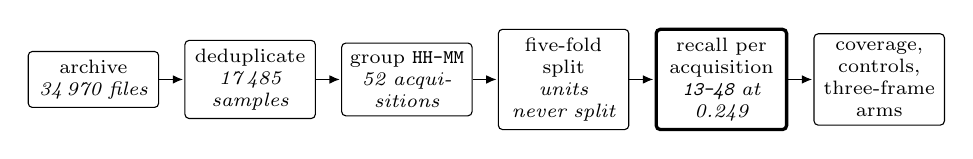
\begin{tikzpicture}[
  bx/.style={draw, rounded corners=1.5pt, align=center, inner xsep=2pt,
             inner ysep=3pt, text width=0.125\textwidth, font=\scriptsize},
  hl/.style={bx, very thick},
  ar/.style={-{Latex[length=1.3mm,width=1.1mm]}, shorten >=0.5pt}]
\node[bx] (a) {archive\\{\itshape 34\,970 files}};
\node[bx, right=3.2mm of a] (b) {deduplicate\\{\itshape 17\,485 samples}};
\node[bx, right=3.2mm of b] (c) {group \texttt{HH-MM}\\{\itshape 52 acquisitions}};
\node[bx, right=3.2mm of c] (d) {five-fold split\\{\itshape units never split}};
\node[hl, right=3.2mm of d] (e) {recall per acquisition\\{\itshape \texttt{13-48} at 0.249}};
\node[bx, right=3.2mm of e] (f) {coverage, controls,\\three-frame arms};
\draw[ar] (a) -- (b); \draw[ar] (b) -- (c); \draw[ar] (c) -- (d);
\draw[ar] (d) -- (e); \draw[ar] (e) -- (f);
\end{tikzpicture}
\caption{Preparation and evaluation. The bold step is the one a frame-level protocol does not produce, and it is free: every unit is held out exactly once, so one cross-validation pass yields a recall per acquisition, and that breakdown exposes \texttt{13-48}.}
\label{fig:pipeline}
\end{figure*}


The database was collected with an FMCW system at 8.75\,GHz with 500\,MHz of bandwidth; the antenna configuration and the rest of the front end are described in the system paper~\cite{quevedo2019}. The published parameters give a range resolution of 0.878\,m, a maximum unambiguous range of 3.598\,km and a Doppler resolution of 0.34\,km/h with 512 integrated ramps. We quote these rather than recomputing them: a naive calculation from bandwidth alone gives a range resolution roughly three times finer than the system achieves.

Samples are supplied as $11 \times 61$ matrices obtained by applying a constant false alarm rate detector to the full range--Doppler matrix and cropping around each detection. The retained Doppler window spans about 21\,km/h, narrower than the extent associated with rotor blade returns from a small rotorcraft, so the crops cannot support blade-flash analysis, which constrains the mechanism arguments available.

\subsection{Recovering acquisition structure}

The distributed archive carries the directory tree twice, once beneath a \texttt{data/} prefix and once at the root, so a naive load doubles every sample. Folder hashing removes the copies and leaves 5720 vehicle, 5065 drone and 6700 pedestrian samples, 17\,485 in all, matching the published figure exactly~\cite{zhang2025}; the digest and the guard against truncated copies are in the artefact.

Acquisition structure is encoded in the directory hierarchy rather than in file names, which are running indices: folders are named by acquisition time, with suffixes distinguishing variants recorded in the same session, for example \texttt{15-55}, \texttt{15-55a}, \texttt{15-55m} and \texttt{15-55p}. We group by the leading \texttt{HH-MM} timestamp, which is a fact about when the data was collected and cannot drift with a parameter choice, and which yields 15 vehicle, 21 drone and 16 pedestrian units, 52 in total, from 80 folders.

We call a timestamp group an \emph{acquisition} throughout, as shorthand for a proposed grouping unit: the rule is an inference from directory structure, not a ground-truth identifier. The suffix pattern is systematic, and several suffixed pairs share a file count \emph{and} peak-to-floor statistics identical to one decimal place, for instance \texttt{17-09} and \texttt{17-09p} at 140 files and 41.4\,dB; every such pair falls within one unit. Merging cannot introduce train/test correlation that folder-level grouping would have avoided, though it does change fold composition. The choice does not reach the principal result: the rule merges folders only in the vehicle class, 27 into 15, and the pedestrian class, 32 into 16, while all 21 drone folders map one to one onto 21 units, so folder-level and timestamp-level grouping are identical for the drone class and \texttt{13-48} is a single folder under either rule.
% =====================================================================
\section{Model and Protocol}
\label{sec:baseline}

\subsection{Architecture and hyperparameters}


\begin{table}[!tb]
\caption{Architecture and training protocol. Strides are (range, Doppler).
Parameter counts are measured: 101\,139 single-frame, 102\,291 three-frame.}
\label{tab:arch}
\centering
\scriptsize
\setlength{\tabcolsep}{3pt}
\begin{tabular}{@{}ll@{}}
\toprule
\multicolumn{2}{@{}l}{\textbf{Network}} \\
\midrule
Input & $11 \times 61 \times 1$ (3 channels in Sec.~\ref{sec:inputgap}) \\
Stem & $3\times3$ conv, 64 ch, stride 1, batch norm, ReLU \\
Stages & separable 64--128 (1,2); 128--208 (2,2); 208--288 (1,2) \\
Separable block & $3\times3$ depthwise, $1\times1$ pointwise, BN, ReLU \\
Head & global mean, dropout 0.2, linear 288 to 3 \\
Parameters & 101\,139 (published reference: 101\,419) \\
\midrule
\multicolumn{2}{@{}l}{\textbf{Training}} \\
\midrule
Optimiser & AdamW, weight decay $10^{-4}$ \\
Schedule & one-cycle, peak rate $3\times10^{-3}$ \\
Batch, epochs & 128; 40 with early stopping, patience 10 \\
Model selection & best validation epoch, restored \\
Loss & cross entropy, unweighted \\
Validation data & whole held-back units, never frames \\
Normalisation & fixed affine offset, $(x+60)/60$, $x$ in dB \\
\bottomrule
\end{tabular}
\end{table}

We use a compact depthwise-separable convolutional network of 101\,139 parameters, set out in full in Table~\ref{tab:arch}, sized to match the 101\,419-parameter reference model reported on this dataset~\cite{zhang2025} so that its behaviour is representative of a network that would plausibly be deployed.

Input normalisation was selected by ablation over grouped folds at seed 0, before any per-acquisition analysis. A fixed affine offset reached 0.925 accuracy against 0.908 for peak-referenced normalisation, with global standardisation and a two-channel peak-plus-level scheme both at 0.922. Being a fixed affine map, it also keeps the artefact's compression analysis interpretable, since quantising before or after it is equivalent up to a scale factor. Width and schedule were set the same way, by a sweep over three width multipliers and two epoch budgets reported in Section~\ref{sec:inputgap}; the best of the six improves on the configuration used here by 0.0009.

\subsection{Partitioning}

Under the \emph{grouped} protocol, whole timestamp units are assigned to train, validation, or test; no unit contributes samples to more than one subset. Folds are balanced by sample count rather than unit count, since unit sizes range from 31 to 660 files. Under the \emph{random} protocol, individual frames are shuffled, with fold sizes matched per class to the
grouped folds.

A seed sets the partition as well as the initialisation, drawing the validation units within a fold and, in the held-out experiments, the train/validation division of the remaining pool, so seeds are randomisation replicates over both. Validation data is drawn from whole training units, never from training frames: validating on random frames under a grouped protocol would reintroduce the correlation the protocol exists to remove. Splits are verified by content hash rather than by path, duplicate folders making path-level verification unsound.

% =====================================================================
\section{What Does Random Partitioning Hide?}
\label{sec:leak}

We ran five folds by three seeds under each protocol, separating two sources of variation: \emph{fold} standard deviation measures sensitivity to which units are held out, \emph{seed} standard deviation sensitivity to initialisation alone. Grouped partitioning gives mean accuracy 0.9099 against 0.9335 and mean drone recall 0.8376 against 0.9358. Those differences are not trivial, but they are small beside the fold-to-fold spread: the grouped fold standard deviation is 0.0427 for accuracy and 0.1389 for drone recall, roughly eight and eighteen times the random-partition figures of 0.0055 and 0.0078, while seed standard deviations stay below 0.04 throughout.

We rest no claim on a significance test. Fold scores under the two protocols are not naturally paired, since a grouped fold is defined by which acquisitions it contains while a random fold is defined by a shuffle, and cross-validation scores are dependent through overlapping training sets~\cite{dietterich1998,nadeau2003}. \textbf{We therefore report that we did not establish a significant aggregate difference between the protocols, which is a weaker statement than the absence of one.} What the data shows clearly is heterogeneity: the per-fold differences in drone F1 are $+0.003$, $-0.023$, $+0.007$, $-0.226$ and $-0.010$, so the aggregate difference is dominated by a single fold rather than appearing as a consistent shift. Section~\ref{sec:regime} identifies what that fold contains.

% =====================================================================
\section{One Acquisition Behaves Differently}
\label{sec:regime}

\subsection{Per-session recall}

Recalls for \texttt{13-48} differ below because the training and test sets differ: cross-validation tests the whole acquisition as one out-of-fold fold (0.249), the coverage test a held-back half (0.178), and Section~\ref{sec:inputgap} excludes it from training entirely (0.238 at one frame, 0.367 at three). We name the protocol wherever a figure appears.


Because every unit appears in the test fold exactly once, a single cross-validation pass yields an out-of-fold recall for each of the 52 acquisitions. Across drone acquisitions, twenty fall above 0.90, between 0.9006 and 0.9929. One, \texttt{13-48}, is classified at 0.249 (grouped CV). The weakest pedestrian and vehicle acquisitions are 0.7776 and 0.8189, respectively.

Excluding \texttt{13-48}, the standard deviation of drone recall across acquisitions is 0.0269, \emph{lower} than that of vehicles (0.0522) or pedestrians (0.0567). The drone class does not generalise poorly in general: the apparent effect, and the outlying fold in Section~\ref{sec:leak}, are both dominated by a single acquisition.

\subsection{What distinguishes it}

We profiled twelve per-sample properties and computed for each the standardised difference $d = (\bar{x}_{\mathrm{13\text{-}48}} - \bar{x}_{\mathrm{others}}) / s_{\mathrm{others}}$, the gap in units of the spread among the other drone acquisitions, a descriptive effect size rather than a test statistic. Only five properties exceed $|d|=2$, and two dominate: Doppler centroid, at bin 8.50 against 30.04 ($d=-15.67$), and peak Doppler bin, 7.58 against 30.01 ($d=-8.16$); the remaining three, headroom, peak level and dynamic range, fall between $+2.07$ and $+2.57$. Range position, range spread and energy extent are unremarkable, so the separation is almost entirely in Doppler position.

\begin{figure}[t]
\centering
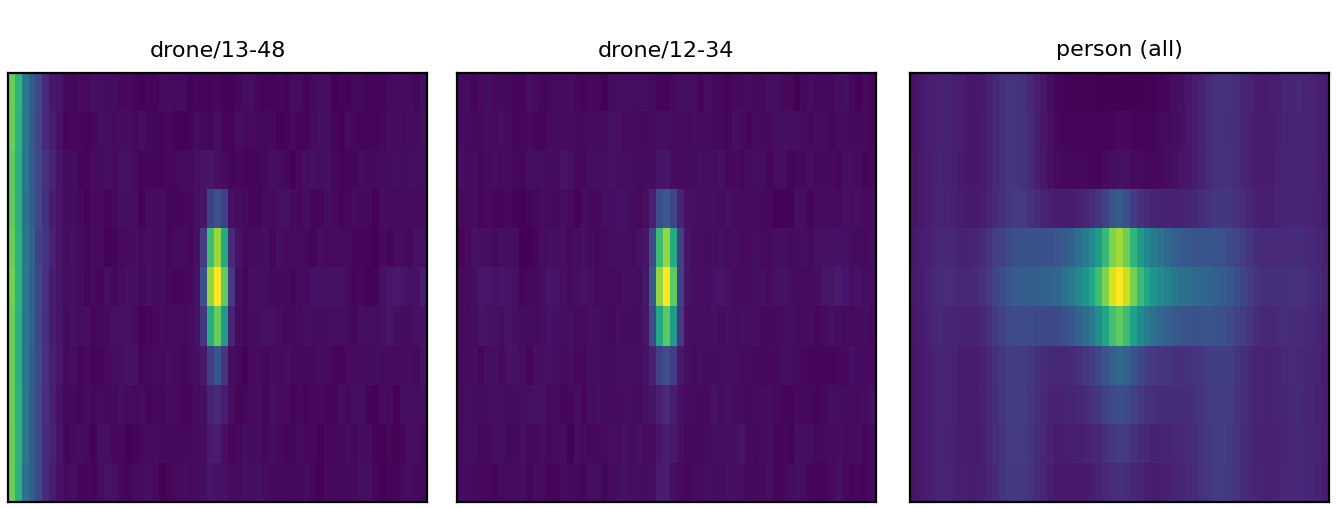
\includegraphics[width=0.82\columnwidth]{session_13-48_compact.png}
\caption{Acquisition means, range vertical and Doppler horizontal.
\texttt{13-48} carries a band of energy at the low edge of the retained
Doppler window that no typical drone acquisition shows, and the pedestrian
mean spreads along that axis, which is where 79\,\% of held-out
\texttt{13-48} goes.}
\label{fig:sessions}
\end{figure}


\begin{figure}[!tb]
\centering
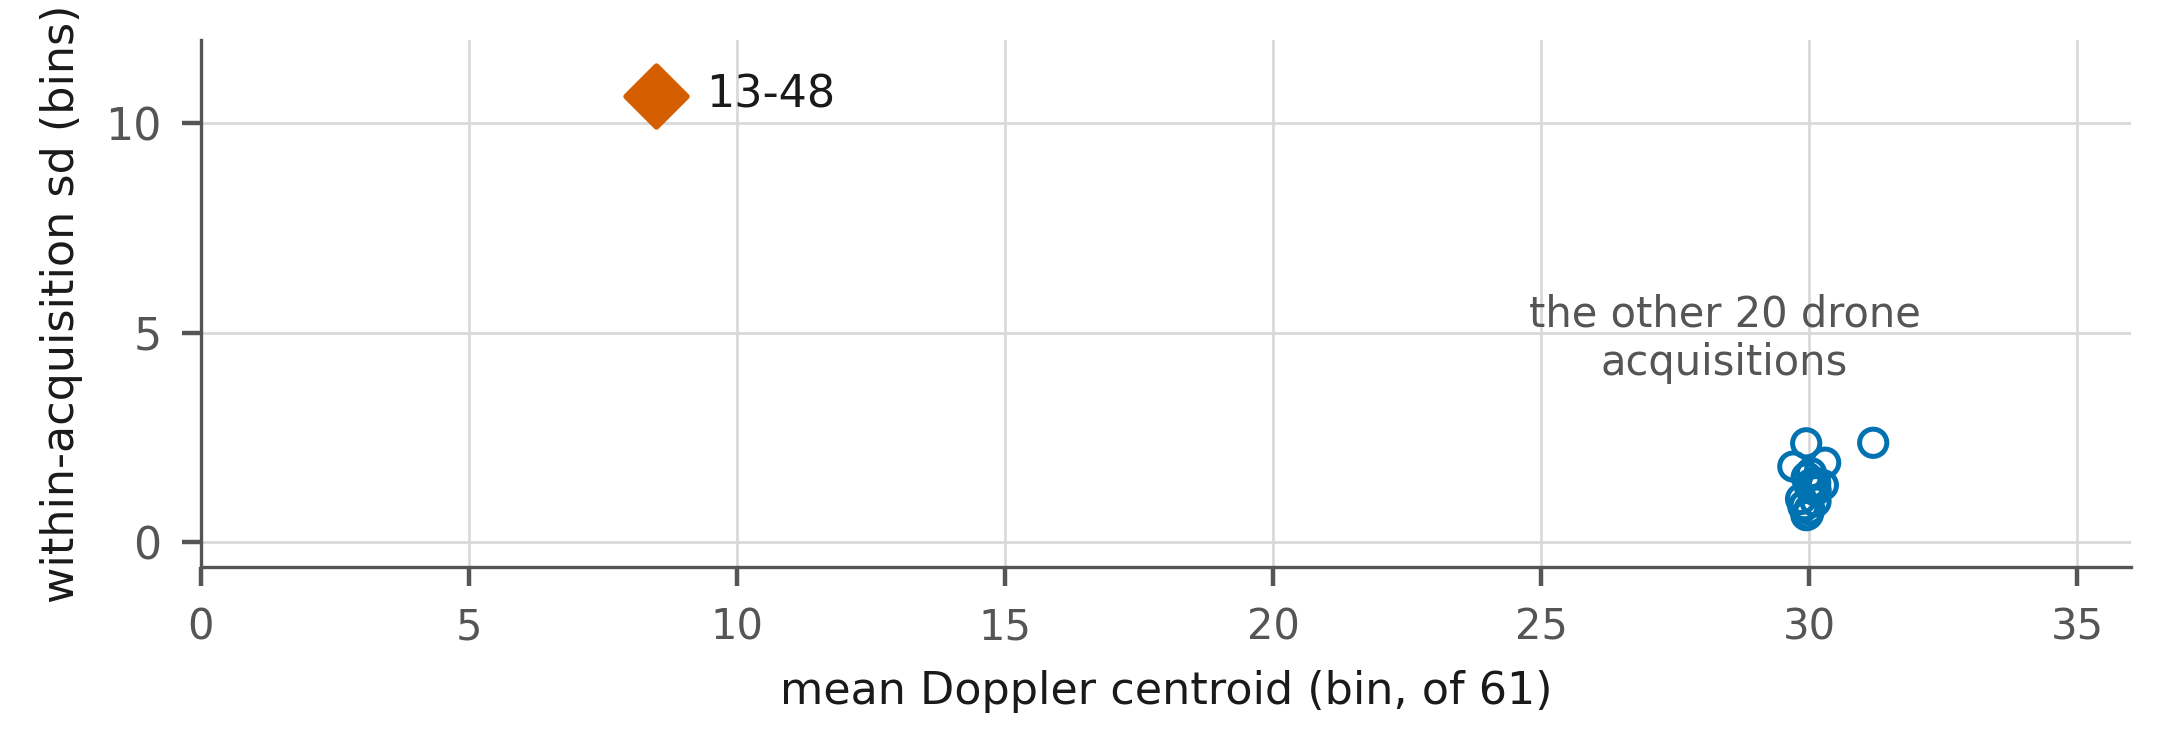
\includegraphics[width=\columnwidth]{doppler_by_acquisition.png}
\caption{The 21 drone acquisitions by Doppler centroid and by its spread
within the acquisition. Twenty cluster at 29.70 to 31.19 with spreads of 0.64
to 2.37 bins; \texttt{13-48} sits at 8.50 with a spread of 10.64, separated
on both axes at once.}
\label{fig:doppler}
\end{figure}

Fig.~\ref{fig:doppler} gives the two-dimensional view. Every other drone acquisition places its target energy at Doppler centroid between 29.7 and 31.2, the centre of the 61-bin axis, and holds it there within 0.64 to 2.37 bins. Acquisition \texttt{13-48} places it at 8.50 with a standard deviation of 10.64, four and a half times the largest any other shows, so it is separated both on where its energy sits and on how much that position varies. Against class centroids from the other acquisitions, 100\,\% of its samples sit nearest the drone centroid, consistent with the label rather than evidence for it.

The source publication describes three drone exercises: radial trajectories on autopilot to 3.1\,km, a circular trajectory at 800\,m, and a free flight with speed and altitude varied manually~\cite{roldan2020,quevedo2019}. Manual free flight can produce more variation in radial velocity than an autopilot trajectory, and \texttt{13-48} is the only acquisition whose Doppler scatter is an order of magnitude above the rest, so we consider it the likeliest candidate, though the publication gives no timestamps and a per-recording processing difference cannot be excluded.

\subsection{Coverage test}

To separate absence of comparable training data from intrinsic difficulty, we split \texttt{13-48} in half. In the first condition, the acquisition is excluded from training entirely and the model is evaluated on one half; in the second, the other half is added to the training set.


\begin{table}[t]
\caption{Coverage test, mean of ten seeds. Each acquisition is first excluded
from training entirely, then half of it is added back; both conditions are
evaluated on the same held-back half. The two controls were selected after
observing per-acquisition recall and are therefore exploratory.}
\label{tab:coverage}
\centering
\small
\setlength{\tabcolsep}{4pt}
\begin{tabular}{@{}llccc@{}}
\toprule
Acquisition & Class & Held out & Half in training & Recovery \\
\midrule
\texttt{13-48} & drone      & 0.178 & \textbf{0.948} & \textbf{$+0.770$} \\
\texttt{11-23} & pedestrian & 0.800 & 0.856          & $+0.056$ \\
\texttt{15-37} & vehicle    & 0.837 & 0.845          & $+0.008$ \\
\bottomrule
\end{tabular}
\end{table}

Both conditions are evaluated on the same held-back half ($N=197$). Recall rises from 0.178 to 0.948 over ten seeds, a recovery of 0.770 (coverage test, Table~\ref{tab:coverage}). Held out, 79\,\% of samples are assigned to the pedestrian class; with half the acquisition in training, 3\,\% are. Held-out recall ranges 0.142 to 0.264 and the half-in-training condition 0.904 to 0.980, so the worst seed of one still exceeds the best of the other by 0.640, a separation that assumes nothing about either distribution.

The failure is therefore associated with the absence of comparable training examples rather than an irreducible inability to classify such samples, though we stop short of a stronger causal statement: because the added samples come from the same acquisition, the experiment cannot separate an out-of-distribution flight regime from an acquisition-specific signature or a per-recording processing difference. It establishes that something present here and absent from the other twenty is learnable and sufficient.

\subsection{Every acquisition, not three}
\label{sec:controls}

\begin{figure}[!tb]
\centering
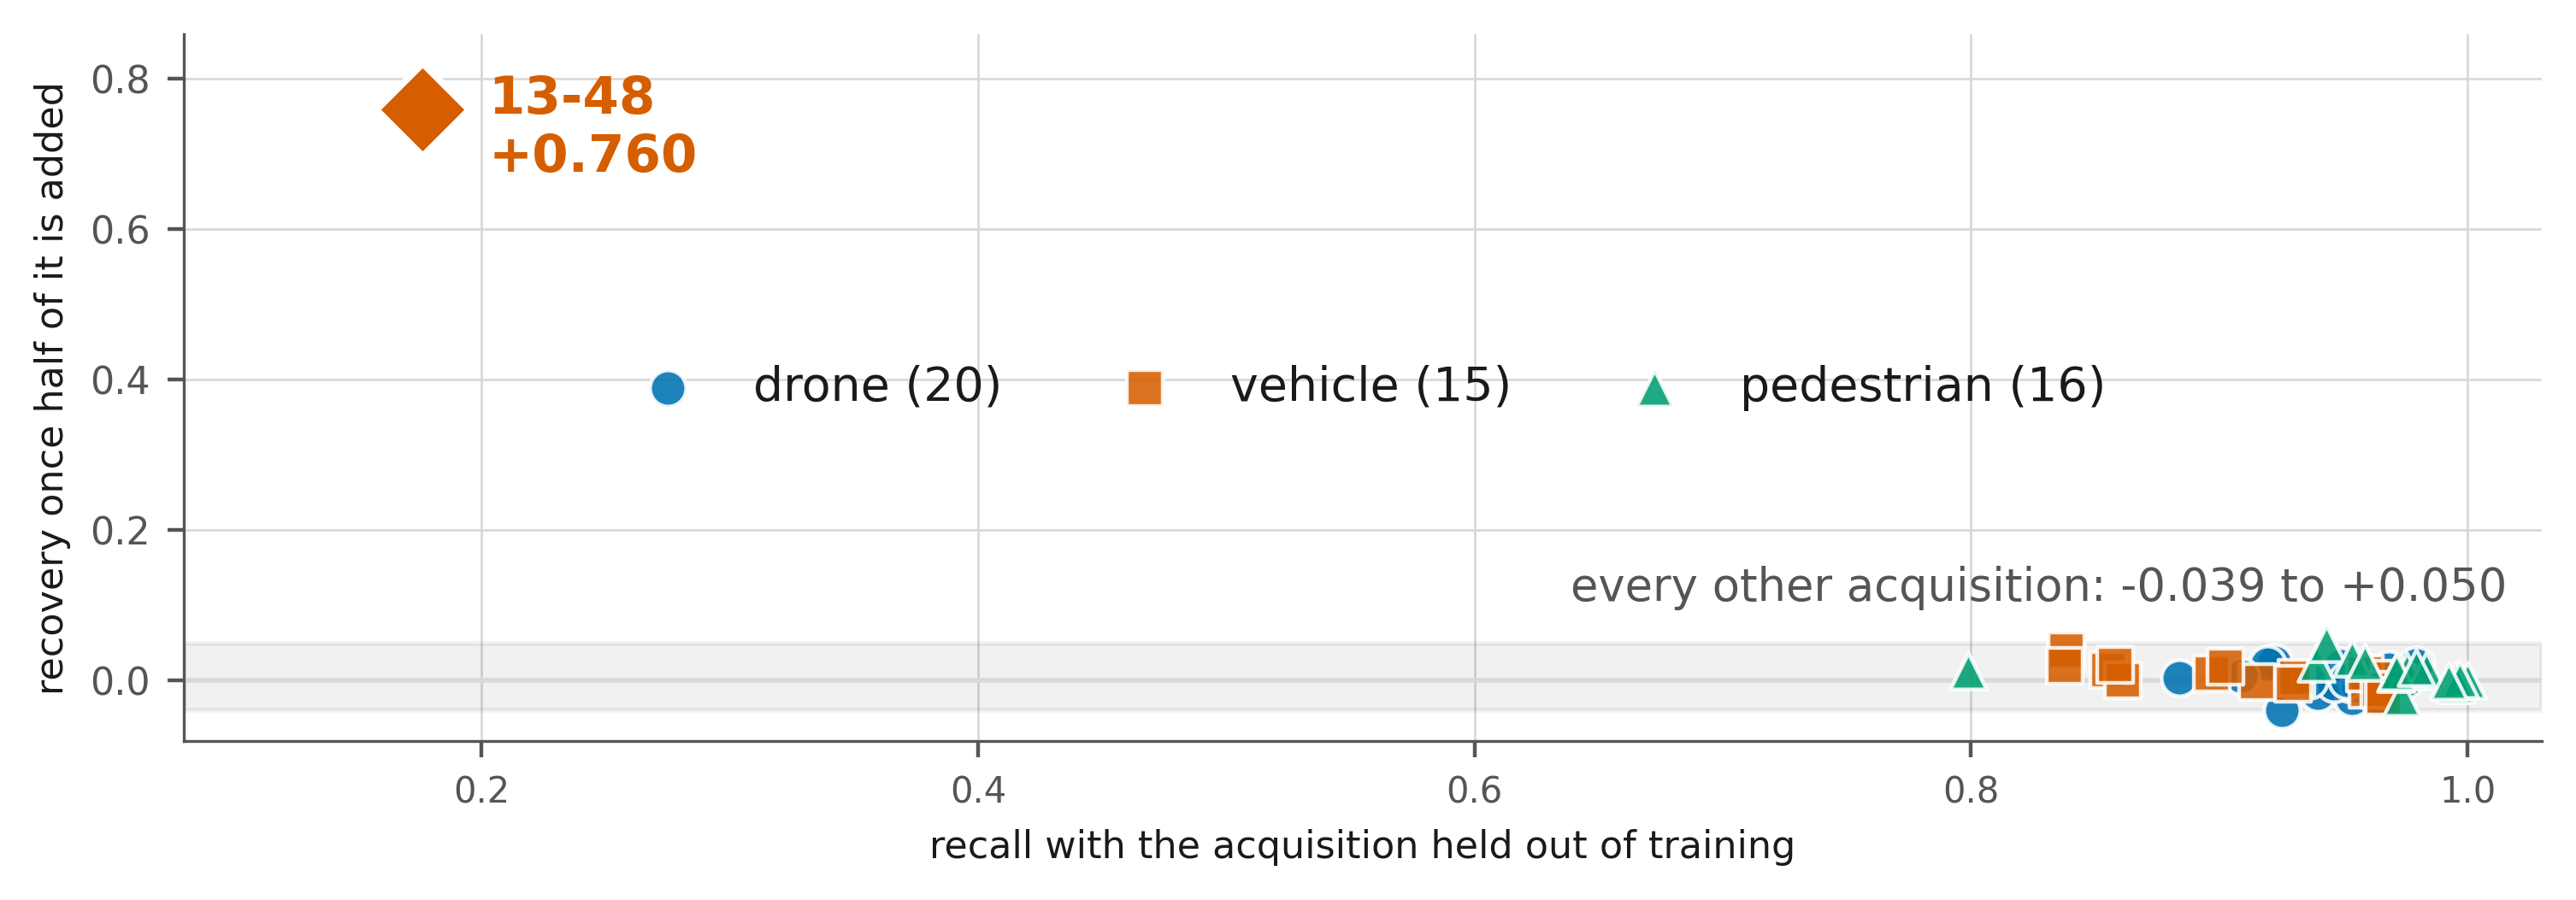
\includegraphics[width=\columnwidth]{recovery_by_acquisition.png}
\caption{The coverage test run on all 52 acquisitions at three seeds:
recovery against the recall the unit reaches while held out. The $x$ axis
doubles as the per-acquisition breakdown: the other 51 all reach at least
0.79 held out and all fall in the shaded band, $-0.039$ to $+0.050$.
\texttt{13-48} recovers $+0.760$, fifteen times the largest any other
reaches, and among the other 51 the two axes are only weakly associated
($r=-0.28$).}
\label{fig:recovery}
\end{figure}

A large recovery is evidence of a coverage failure only if a large recovery
is unusual. Rather than argue that from acquisitions chosen after seeing
which scored worst, we ran the identical experiment on all 52 units at three
seeds, 312 trainings (Fig.~\ref{fig:recovery}). With \texttt{13-48} set
aside the other 51 span $-0.039$ to $+0.050$, sd 0.017, so \textbf{not one
recovers as much as 0.05}, while \texttt{13-48} recovers 0.760, fifteen
times the largest and far outside anything the rest reach. Among the 20
other drone units the largest is 0.024, and sixteen of the 51 recover
negatively, which is what noise around zero looks like.

The alternative is regression to the mean: a unit scoring badly held out has
more room to improve, so a large recovery might follow from a low starting
point alone. The $x$ axis of Fig.~\ref{fig:recovery} tests it. Across all 52
units baseline recall and recovery correlate at $r=-0.927$, but
\texttt{13-48} alone produces that; among the other 51 it is $-0.282$
($t=-2.06$, 49 d.f.), eight per cent of the variance, and among the 23 units
below 0.95, which have room to move, $-0.238$. A weak association exists and
we report it, but it is nowhere near enough to generate 0.760.

The weakest unit of each other class was additionally examined at ten
seeds: \texttt{11-23} ($N=154$) recovers 0.056 and \texttt{15-37} ($N=185$)
0.008. Neither is unrepresented as \texttt{13-48} is. \texttt{11-23} is an
outlier in extent ($d=+3.4$) with 56.8\,\% of its frames nearest the
\emph{drone} centroid, confusable with another class rather than missing
from training, and no property separates \texttt{15-37} from other vehicle
acquisitions at all. An acquisition can be weak without being
unrepresented, which is the alternative the coverage experiment excludes.

This is the paper's principal result, and it concerns this benchmark: a
classifier whose aggregate score looks healthy fails severely on one of the
dataset's acquisitions, the evidence points to an acquisition-specific
coverage failure rather than a class-wide difficulty effect, and no other
acquisition in the dataset behaves this way. What
that acquisition represents we cannot settle. The release crops a window
around each detection without recording its absolute Doppler reference, so
the displacement is low \emph{relative} Doppler within the crop rather than
a measured velocity, and it could follow equally from flight dynamics or
from a recording-specific processing difference. A
deployment consequence follows only under the first reading, so we state the
evaluation finding and leave the physical one open.

% =====================================================================
\section{Discussion and Limitations}
\label{sec:discussion}

\subsection{What the results do and do not support}

The coverage result is the finding we consider established: an effect of 0.77 in recall, a controlled manipulation isolating within-acquisition coverage, and a sweep over all 52 units placing it far outside the rest. It does not identify which physical or processing factor makes that coverage necessary. Where deployment operates on the benchmark's own distribution, frame-level evaluation may be appropriate.

A compression study in the artefact found that fourfold Doppler aggregation raises held-out recall on \texttt{13-48} from 0.222 to 0.398 on ten of ten seeds with no change on the standard split, but helped only three of five acquisitions tested singly, so it is acquisition-specific rather than a recommendation.

Four physically motivated mechanisms were formulated and none was supported: rotor sideband loss, which the crops' Doppler span does not let us assess; low redundancy from compact energy; limited dynamic-range headroom, whose correlation with per-acquisition recall (Pearson $-0.62$) falls to $-0.16$ once \texttt{13-48} is excluded, that acquisition having the largest headroom of any at 42.5\,dB against a class median near 26; and Doppler positional insensitivity, which shift augmentation at $\pm 4$, $\pm 8$ and $\pm 16$ bins fails to repair, giving 0.1608, 0.1613 and 0.1603 against 0.2214 unaugmented. None supports an explanation; none excludes the physics our data cannot reach.

\subsection{Limitations}

Both principal findings rest on the same acquisition, so the effective sample size at the level of flight regimes is one, from one dataset, one radar and one drone platform, with \texttt{13-48} comprising 7.8\,\% of the drone samples. The coverage claim is no longer a contrast of hand-picked cases, but a distribution over 52 units of one dataset still says nothing about how common such acquisitions are elsewhere, and that sweep runs at three seeds against ten for the focal experiment. Whether the phenomenon appears under other architectures, or on another radar, is untested here. Two changes to our own model leave it in place: widening to 871\,731 parameters and supplying three-frame input both raise aggregate accuracy without lifting this acquisition above 0.367. That points to a property of what the training split covers rather than of capacity or input length, and we would expect the failure to survive a change of architecture, but we have not shown it.

\subsection{Approximate temporal context, and what it does not show}
\label{sec:inputgap}

The experiments in this subsection use our own compact network with an approximate three-frame input. They do not reproduce DopplerNet and say nothing about how it would perform on \texttt{13-48}. Our classifier reaches 0.9335 under grouped five-fold cross-validation and 0.9537 on a single random partition, against the 99.48\,\% reported for DopplerNet and the 98.08\,\% for the lighter reference. The three numbers do not measure the same thing, and the differences run in opposite directions.

DopplerNet's figure is a five-fold cross-validated mean over five random subsets~\cite{roldan2020}, the same protocol as our 0.9335, so the comparison is like for like and the gap is 6.1 points, none of which protocol explains. Two documented differences remain: DopplerNet has 3\,818\,755 parameters against our 101\,139, and its input is an $11 \times 61 \times 3$ distance-Doppler-time tensor, three consecutive detections stacked as channels 400\,ms apart. Our model, and every experiment above, sees one frame.

The lighter reference differs in the other direction. Its 0.9808 is a peak validation accuracy on an 80/20 split with no separate test set~\cite{zhang2025}: the best epoch's accuracy, measured on the data used to choose that epoch. Our 0.9537 is test accuracy on data withheld from both training and model selection, and that architecture is within three hundred parameters of ours on the same single-frame input. The two quantities are not comparable, and we report ours at the more conservative definition.

Capacity and schedule explain nothing at this scale: across width multipliers of one, two and three, to 871\,731 parameters, and 40 and 80 epochs, the best of the six reaches 0.9546, only 0.0009 above the network we use.

Nor can a user of the release remove that difference. The archive supplies one CFAR-cropped matrix per detection with no timestamp and no frame counter, the only ordering being the trailing integer in each file name. The 400\,ms triplets are therefore not reconstructible from the public data by anyone, so a headline accuracy obtained from an input the release does not retain cannot be reproduced from it. That is a reporting problem of the same family as the one studied here.

We can nevertheless approximate that formulation and test whether the approximation carries temporal information. Triplets form within each folder from consecutive file-name integers, never across a gap, giving 17\,221 triplets from 17\,485 frames and 391 on \texttt{13-48}. Four arms are compared at ten shared seeds on the same triplet centres, so the comparison is paired sample for sample (Table~\ref{tab:temporal}): \emph{single}, the centre alone; \emph{index}, its two index-adjacent neighbours; \emph{clean}, the nearest neighbours carrying the centre's own split tag, so no window crosses the partition; and \emph{shuffle}, two frames drawn at random from the same folder, a transductive context rather than a deployable one. All three multi-frame arms hold channel count, folder, labels and sample count fixed, and three channels take the model from 101\,139 to 102\,291 parameters.

\begin{table}[t]
\caption{Approximate three-frame context, ten seeds; random-split figures
are three seeds. $d$ is the mean index distance of the companion frames from
the centre. This is our own network, not DopplerNet. $^{\dagger}$The shuffle
arm draws companions from anywhere in the folder, including other test
frames, so it is transductive and its 0.9932 is not deployment-comparable.}
\label{tab:temporal}
\centering
\small
\setlength{\tabcolsep}{3pt}
\begin{tabular}{@{}llccc@{}}
\toprule
Arm & Companions & $d$ & Random split & \texttt{13-48} recall \\
\midrule
single  & none            & --   & 0.9516 $\pm$ 0.0046 & 0.2379 $\pm$ 0.0428 \\
index   & adjacent        & 1.00 & 0.9794 $\pm$ 0.0016 & 0.3673 $\pm$ 0.0661 \\
clean   & same split tag  & 2.57 & 0.9731 $\pm$ 0.0080 & 0.4634 $\pm$ 0.0970 \\
shuffle$^{\dagger}$ & folder-wide & -- & 0.9932 $\pm$ 0.0016 & 0.5435 $\pm$ 0.1257 \\
\bottomrule
\end{tabular}
\end{table}

A three-frame input raises random-split accuracy from 0.9516 to 0.9794, within a quarter of a point of the 0.9808 reported for the lighter published model. That classifier still fails on \texttt{13-48}: recall rises from 0.238 (single frame, held out) to 0.367 (three-frame index arm, held out), a paired gain of $+0.129$ over ten seeds ($t=+4.82$), so most of the acquisition's frames are still assigned to the wrong class. \textbf{The failure is therefore not an artefact of the single-frame input, and it persists while aggregate accuracy rises by 2.8 points.} Even the shuffle arm at 0.9932 leaves it at 0.544, far below the 0.948 obtainable once it is represented in training.

The second result we did not anticipate. A sliding window over a frame-level random split does put test frames inside training inputs on a large scale: 50.6\,\% of training triplets hold at least one, and 82.7\,\% of all test frames appear inside some training input under index order against 68.4\,\% under shuffled companions. The \emph{clean} arm, which the audit reports at exactly zero overlap, measures what that is worth: removing the overlap costs 0.0063 in accuracy, 0.9794 against 0.9731, inside the spread of either arm. So although four fifths of the test set appears somewhere in training, the inflation is well under a point here, and three frames still beat one by 0.0215 with no overlap at all. We report it in both directions because the audit alone would have supported a stronger claim than the experiment does.

What separates the arms is how far the companions sit from the centre. Recall on \texttt{13-48} rises monotonically with that distance: 0.367 for index-adjacent frames, 0.463 for the nearest same-tag frames at a mean distance of 2.57, and 0.544 for companions drawn from anywhere in the folder. Adjacent detections are nearly redundant, while more distant ones sample the acquisition's variability, largest precisely here (Section~\ref{sec:regime}). The shuffle arm is additionally transductive, drawing on other test frames at inference as a live system could not, so \emph{index} is the arm the comparison rests on. Even index is not causal with respect to its own centre, since the window is centred on the frame being classified: a streaming system could form it only by delaying each decision by one frame, the latency the source publication notes for its own three-frame input~\cite{roldan2020}. We therefore call it temporally ordered adjacent-frame context, not a deployment-ready one. Index and shuffle differ by 0.176 ($t=-4.35$ over ten paired seeds) rather than by chance, so the trailing integer tracks acquisition order closely enough to matter.

\section{Conclusion}

On the Real Doppler RAD-DAR benchmark, grouping by inferred acquisition exposes heterogeneity that aggregate frame-level accuracy does not show. One drone acquisition of twenty-one attains 0.249 out-of-fold recall against 0.90 or better for the other twenty; excluded from training entirely it reaches 0.178 on a held-back half and 0.948 once the other half is added. The same experiment on all 52 units leaves it alone: no other recovers as much as 0.05. It differs sharply in Doppler position and variability, though the release carries no metadata separating flight dynamics from a recording-specific processing condition, and the failure persists in our compact classifier when three-frame context is added.

These results are a benchmark-specific case study rather than a general law, but they do support reporting acquisition-level performance wherever a dataset is assembled from continuous recordings, since it costs one cross-validation pass. Code, partition files, per-stage reports and a script that rechecks every number here against its own tolerance are released at \codeurl{}~\cite{dataset2026}.

% =====================================================================
\begin{thebibliography}{00}

\bibitem{roldan2020} I.~Roldan, C.~R.~del-Blanco, \'A.~Duque de Quevedo \emph{et al.}, ``DopplerNet: a convolutional neural network for recognising targets in real scenarios using a persistent range--Doppler radar,'' \emph{IET Radar Sonar Navig.}, vol.~14, no.~4, pp.~593--600, 2020.

\bibitem{quevedo2019} \'A.~Duque de Quevedo, F.~Ib\'a\~nez Urzaiz, J.~Gismero Menoyo \emph{et al.}, ``Drone detection and radar-cross-section measurements by RAD-DAR,'' \emph{IET Radar Sonar Navig.}, vol.~13, no.~9, pp.~1437--1447, 2019.

\bibitem{zhang2025} L.~Zhang, G.~Tu, Y.~Xu \emph{et al.}, ``A lightweight CNN for micro-Doppler UAV detection and classification,'' \emph{Electronics}, vol.~14, no.~24, art.~4831, 2025.

\bibitem{kim2016} Y.~Kim and T.~Moon, ``Human detection and activity classification based on micro-Doppler signatures using deep convolutional neural networks,'' \emph{IEEE Geosci. Remote Sens. Lett.}, vol.~13, no.~1, pp.~8--12, 2016.

\bibitem{ahmad2023} B.~I.~Ahmad, C.~Rogers, S.~Harman \emph{et al.}, ``A review of automatic classification of drones using radar: key considerations, performance evaluation and prospects,'' \emph{IEEE Aerosp. Electron. Syst. Mag.}, 2023, doi:10.1109/MAES.2023.3335003.

\bibitem{kapoor2023} S.~Kapoor and A.~Narayanan, ``Leakage and the reproducibility crisis in machine-learning-based science,'' \emph{Patterns}, vol.~4, art.~100804, 2023.

\bibitem{buchman2022} D.~Buchman, M.~Drozdov, T.~Krilavi\v{c}ius \emph{et al.}, ``Pedestrian and animal recognition using Doppler radar signatures,'' \emph{Sensors}, vol.~22, no.~9, art.~3456, 2022.

\bibitem{chen2025} L.~Chen, N.~Zhu, H.~Chen \emph{et al.}, ``A causality-inspired single-source domain generalized method for low-slow-small threat target recognition,'' \emph{Expert Syst. Appl.}, vol.~287, art.~128104, 2025.

\bibitem{bai2026} B.~Bai, L.~Xue, M.~Xue \emph{et al.}, ``Open-set recognition of radar range profiles with attention and multi-task joint training,'' \emph{IET Radar Sonar Navig.}, vol.~20, no.~1, art.~e70121, 2026.

\bibitem{dietterich1998} T.~G.~Dietterich, ``Approximate statistical tests for comparing supervised classification algorithms,'' \emph{Neural Comput.}, vol.~10, no.~7, pp.~1895--1923, 1998.

\bibitem{nadeau2003} C.~Nadeau and Y.~Bengio, ``Inference for the generalization error,'' \emph{Mach. Learn.}, vol.~52, no.~3, pp.~239--281, 2003.

\bibitem{hooker2019} S.~Hooker, A.~Courville, G.~Clark \emph{et al.}, ``What do compressed deep neural networks forget?'' arXiv:1911.05248, 2019.

\bibitem{tran2022} C.~Tran, F.~Fioretto, J.-E.~Kim \emph{et al.}, ``Pruning has a disparate impact on model accuracy,'' in \emph{Adv. Neural Inf. Process. Syst.}, vol.~35, 2022, pp.~17652--17664.

\ifblind
\bibitem{dataset2026} \anon{} ``Code and analysis for this paper,'' archived artefact, 2026. Withheld for blind review.
\else
\bibitem{dataset2026} G.~Mustafa, ``Code and analysis for this paper,'' Zenodo, 2026, doi:10.5281/zenodo.23118075.
\fi

\end{thebibliography}

\end{document}